% Start of the appendix
\appendix
\clearpage

\section{Supplemental Details for \BENCHMARK{}}
\label{appendix-benchmark-supp-details}

% an example for prompts and case study

\subsection{Dataset Construction}
\label{appendix-dataset-construction}

In this section, we discuss the details of our benchmark construction process.

\paragraph{Attribute Ontology} In \Cref{tab:attribute-ontology}, we provide the full attribute ontology used in \BENCHMARK{}.  This attribute ontology is constructed manually to reflect commonly mentioned topics in user-assistant chats. Five major categories are included: demographic information, lifestyle, situational context, life events, and belongings.

\begin{table}[h]
    \centering
    \caption{Human-constructed user attribute ontology. Each attribute represents a unique dimension of human experience along which a user biography could be constructed. For \BENCHMARK{}, we sample user backgrounds based on each of the attributes and construct questions on top of them. }
    \resizebox{\linewidth}{!}{
\begin{tabular}{p{\textwidth}}
    \toprule
    \rowcolor{gray!20} \textbf{Attribute 1: Demographic Information} \\
    age, gender, ethnicity, nationality, language, education level, occupation \\
    \midrule
    \rowcolor{gray!20} \textbf{Attribute 2: Lifestyle} \\
    \textbf{2.1: Shopping}: online shopping frequency, favorite stores, loyalty program, sales events, coupons, gift purchasing habits, eco-friendly product preferences, luxury vs budget shopping, technology gadget purchasing, fashion and apparel, grocery shopping, shopping for others \\
    \textbf{2.2: Media Consumption}: book, movie, tv show, music, podcast, video game, streaming service, theater, magazine and newspaper, youtube, educational content, audiobook and e-book \\
    \textbf{2.3: Social Media Engagement}: posting, commenting, followers, groups, hashtags, campaigns, messaging, live streaming, social media breaks \\
    \textbf{2.4: Daily Routines}: wake-up time, bedtime, work or school start time, meal time, exercise routines, coffee or tea break, commuting, evening activities, weekend routines, cleaning schedules, time spent with family or friends \\
    \textbf{2.5: Travel}: frequency, destination, road trips, travel agencies, outdoor adventures, airlines, hotel, travel with family vs solo travel, packing habits \\
    \textbf{2.6: Recreation}: reading, painting, musical instruments, dancing, watching sports, participating in sports, gardening, bird watching, fishing or hunting, board games, video games, fitness classes, yoga, sculpting, photography, stand-up comedy, writing, collecting, model building, aquarium keeping \\
    \textbf{2.7: Eating and Cooking}: home cooking, food delivery, vegetarian or vegan, favorite cuisines, snacking habits, barbecue, baking, cocktail mixing, cooking classes \\
    \textbf{2.8: Event Participation}: concerts, theater, galleries and museums, sports games, film festivals, religious services, book readings, charity events, trade shows, lectures or workshops, theme parks, local markets, networking events, sports, auto racing, workshops, museum tours \\
    \midrule
    \rowcolor{gray!20} \textbf{Attribute 3: Situational Context} \\
    \textbf{3.1: Home}: living room, kitchen, bathroom, room style, room lighting, furniture, technology, plants \\
    \textbf{3.2: Social Context}: alone, family, friends, interactions with strangers \\
    \textbf{3.3: Time Context}: time of day, day of week, seasonal \\
    \midrule
    \rowcolor{gray!20} \textbf{Attribute 4: Life Events} \\
    graduations, academic achievements, study abroad, significant academic projects, job promotions, starting a business, births and adoptions, marriages, family reunions, illness or surgeries, mental health journeys, purchasing a home, trips, movement, living abroad, refugee or immigration, loss of loved ones, name change, belief, milestone \\
    \midrule
    \rowcolor{gray!20} \textbf{Attribute 5: Belongings} \\
    cars, bikes, vehicles, computer, phone, pet, farm animal, animal care items, home, land, art, antiques, collectible, rare items, clothing, jewelry, shoes, bag, sports gear, musical instruments, health related devices, crafting, photography \\
    \bottomrule
\end{tabular}
}
\label{tab:attribute-ontology}
\end{table}




\paragraph{Background Sampling} Based on each of the attributes, we prompt Llama 3 70B Instruct to generate a background paragraph outlining the user memory and experience. In our preliminary studies, we find that the following zero-shot prompt in \Cref{fig:user-background-prompt} can already guide the model to generate a long and focused user background with sufficient details, which suffices for the next step of question creation. We thus use the same prompt for the final version of \BENCHMARK{}.

\begin{figure*}[t]
 \begin{tcolorbox}
 I will give you a topic. Please imagine you are a user that wants to recall and record recent personal facts along the topic. Generate a long text describing these personal facts. Use your imagination and generate the personal facts. Make it long and involve several recent facts or recent events spanning many days, weeks, or monthes. You may state the facts in plain language and no need to make it story-like.\\
 
 Topic: \{attribute\} \\
 
 Recent Personal Facts related to \{attribute\}:
 
 \end{tcolorbox}
 \caption{The prompt for constructing user backgrounds based on an attribute.}
 \label{fig:user-background-prompt}
\end{figure*}

% \diwu{Need (1) a list of user attributes and (2) the background sampling prompt}

\paragraph{Question Construction} As discussed in \Cref{section-benchmark-creation}, based on the generated user backgrounds, Llama 3 70B Instruct is used to propose question and answers for each question type. Additionally, for the question type \textbf{temporal-reasoning}, \textbf{multi-session reasoning}, and \textbf{single-session-preference}, we use GPT-4o to propose several questions. Nevertheless, we find most of the questions to be unsatisfactory and manually filter and edit most of the questions. In total, approximately 1000 questions were generated for each question type, and the final yield rate is about 5\%. For each question, we then manually decompose the answer into the evidence statements. If the question or the evidence statements involve time mentions, we assign a timestamp to the question and the evidence statements at this stage. Note that if timestamps are specified for the evidence statements at this stage, these timestamps will always be used for corresponding evidence sessions. Otherwise, the timestamps will be randomly assigned at the history construction stage with all the other sessions. 

\begin{figure*}[t]
 \begin{tcolorbox}
 % \textbf{System Prompt:} \\

 % xxxxx

 % \textbf{Prompt:} \\

 I will give you a past memory. Use the memory to act as a normal user to chat with a chat assistant. In the chat, you may ask it to assist you various tasks or ask it about various information. However, make sure that your convey the following fact about you: "\{evidence\_statement\}". In addition, make sure your message is concise (1-2 simple sentences), since the real users often do not bother write a long message. I will provide you with the chat history and the response from the assistant. Directly generate the next response from the user's perspective. You must simulate the tone of a neutral user and do not be overly enthusiastic, verbose, formal, or polite. For conciseness, DO NOT react to the assistant's message with e.g., "thanks" or "I will do that". Instead, directly state the follow-up questions or new questions.\\
 
 Memory: \{background\} \\
 
 Chat History: \\
 
 assistant: Hi! How can I assist you today? \\

 ... (more rounds as the conversation continues) ...
 
 \end{tcolorbox}
 \caption{The prompt for instruction an LLM to act as a user and initiates a task-oriented dialogue with another LLM. Both the background and the evidence statement is provided. This prompt is used for the question type \textbf{single-session}. For the other question types, the prompt components are slightly different but the prompt overall follows the same style. }
 \label{fig:chat-simulation-prompt}
\end{figure*}

\paragraph{Evidence Session Construction} Using the question and the decomposed evidence statements, we use Llama 3 70B Instruct to simulate one user-AI chat history per evidence statement via self-chat. In \Cref{fig:chat-simulation-prompt}, we present an example of the chat simulation prompt, where we ask the user LLM to indirectly mention the evidence statement while avoiding to talk about other evidence statements for the question, if there are any. We include two crucial instructions in the prompt to make sure (1) the evidence statement is provided in an indirect way and (2) the generated messages are concise and thus mimic the style of user messages. On the assistant side, we directly provide the input generated by the user LLM without any prompt engineering. We simulate the chat for 10 round at maximum and stopped prematurely when either side of the LLMs generates an empty sequence indicating the end of the conversation. 

Subsequently, expert annotators manually inspect and edit each of the generated sessions to ensure that (1) the required evidence statements are present in the conversation, (2) no other evidence statements are leaked into the conversation, (3) the evidence statements are provided in a colloquial style, especially for the data and time mentions, and (4) the conversation ends gracefully. In total, roughly 70\% of the sessions are human edited. We note that in a few rare instances, the user LLM fails by assuming the assistant role instead. When these failures are identified, we discard the instance if the conversation cannot be fixed.


\subsection{History Construction}
\label{appendix-haystack-sampling}

In order to construct a coherent and freely extensible chat history, we design a three-staged pipeline that include \textit{session pool construction}, \textit{session sampling}, and \textit{timestamp resolution}.

\paragraph{Session pool construction} For each question, we draw the history sessions from three sources: ShareGPT \citep{zheng2023judging}, UltraChat \citep{ ding2023enhancing}, and the simulated sessions corresponding to other attributes using the same pipeline mentioned in the previous section. This pool ensures that the non-evidence history sessions have similar topic or format as the evidence sessions, while avoiding providing conflicting information that would invalidate the question. 


\paragraph{Session sampling} To sample a history containing $x$ sessions, we randomly sample from the aforementioned three sources and shuffle the sessions together with the question's evidence sessions. For \BENCHMARK{}, we always use the following mixture: 25\% ShareGPT, 25\% UltraChat, and 50\% simulated sessions. If the evidence sessions need to follow a specific order, we swap their orders accordingly after shuffling. 

\paragraph{Timestamp resolution} Finally, we randomly assign timestamps to the session following their order of the history. If the evidence sessions are associated with pre-defined timestamps, we use them as anchors to determine the range of timestamp of the non-evidence sessions preceding or following them. Other wise, we randomly assign tiemstamps in May 2023. 
 

\subsection{Basic Statistics}
\label{appendix-basic-statistics}

{In \Cref{fig:benchmark-basic-stats}, we present the basic statistics of \BENCHMARK, revealing that most questions require evidence from multiple sessions (up to six) and that evidence statements are positioned diversely within sessions, increasing the challenge to the memory design.}


\begin{figure}[h]
    \centering
    \vspace{-5mm}
    \begin{subfigure}{0.35\textwidth}
        \centering
        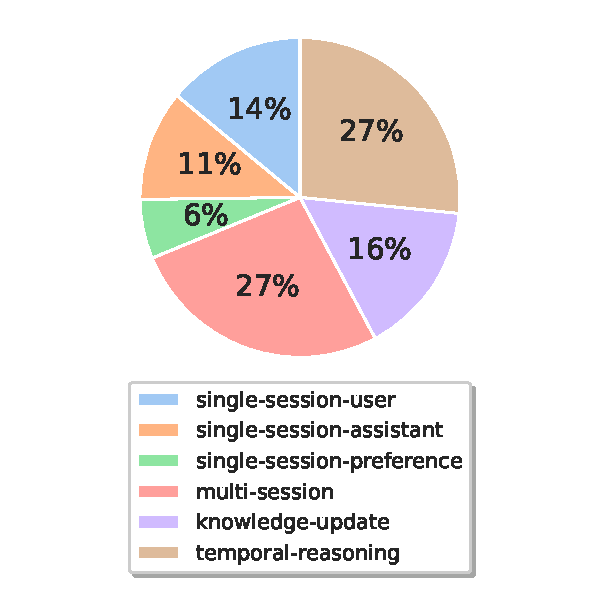
\includegraphics[width=0.9\textwidth]{figures/question_type_distribution.pdf}
        \caption{Distribution of question types in \BENCHMARK{}.}
        \label{fig:subfig2}
    \end{subfigure}
    \hfill
    \begin{subfigure}{0.3\textwidth}
        \centering
        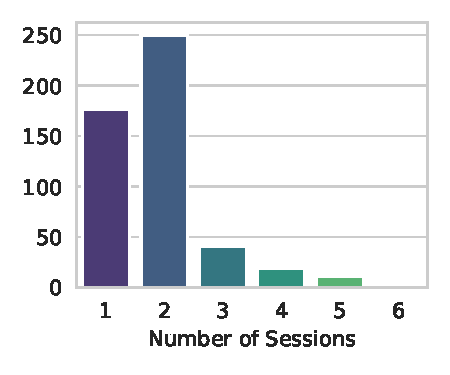
\includegraphics[width=0.9\textwidth]{figures/session_count_distribution.pdf}
        \caption{Distribution of the number of evidence sessions. Most questions emphasize multi-session reasoning, requiring reading up to six sessions to answer.}
        \label{fig:subfig3}
    \end{subfigure}
    \hfill
    \begin{subfigure}{0.3\textwidth}
        \centering
        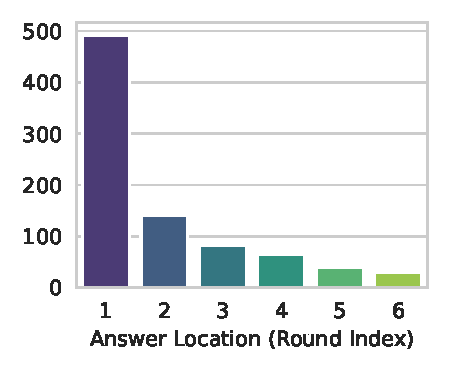
\includegraphics[width=0.9\textwidth]{figures/answer_location_round.pdf}
        \caption{Distribution of the location of the evidence statement within the evidence sessions. Most evidence statements are located at the beginning of the chat.}
        \label{fig:subfig1}
    \end{subfigure}
    % \vspace{-2mm}
    \caption{{\BENCHMARK{} challenges chat assistants through its (a) diverse question types, (b) emphases on multi-session reasoning, and (c) diverse evidence locations within sessions.}}
    % \vspace{-5mm}
    \label{fig:benchmark-basic-stats}
\end{figure}




\subsection{Evaluation Metric Building}
\label{appendix-evaluation–metric}

To accurately evaluate the diverse responses of LLMs, we use an expert-written prompt to instruct GPT-4o as the correctness judge. We present the full prompt in \Cref{fig:evaluation-prompt}. To enable the model to handle detailed edge cases as how expert evaluators would do, we design separate prompts for a number of tasks. To ensure the prompt has a high agreement with expert judge, we sample 30 questions per problem type, collect the long-context generation results from GPT-4o and Llama 3.1 8B Instruct, and report the judgment correctness by category.

As shown in \Cref{tab:meta-evaluation}, the prompt-engineered GPT-4o judge achieves reliable performance in evaluating both GPT-4o and Llama-3.1-8B-Instruct as the generation model. The evaluator's judgment slightly deviates from human experts for the single-session-preference and abstention problems due to the open-ended nature of the response. Nevertheless, our evaluation prompt still achieves 90\% or higher accuracy under all settings. We will include this prompt in the benchmark package that we will release to enable consistent comparisons for future work.


\begin{figure*}[htb]
    \begin{tcolorbox}
    \textbf{temp-reasoning} \\

    I will give you a question, a correct answer, and a response from a model. Please answer yes if the response contains the correct answer. Otherwise, answer no. If the response is equivalent to the correct answer or contains all the intermediate steps to get the correct answer, you should also answer yes. If the response only contains a subset of the information required by the answer, answer no. In addition, do not penalize off-by-one errors for the number of days. If the question asks for the number of days/weeks/months, etc., and the model makes off-by-one errors (e.g., predicting 19 days when the answer is 18), the model's response is still correct. \\

    \hrule
    \bigskip
    
    \textbf{knowledge-update} \\
    
    I will give you a question, a correct answer, and a response from a model. Please answer yes if the response contains the correct answer. Otherwise, answer no. If the response contains some previous information along with an updated answer, the response should be considered as correct as long as the updated answer is the required answer. \\

    \hrule
    \bigskip

    \textbf{single-session-preference} \\
    
    I will give you a question, a rubric for desired personalized response, and a response from a model. Please answer yes if the response satisfies the desired response. Otherwise, answer no. The model does not need to reflect all the points in the rubric. The response is correct as long as it recalls and utilizes the user's personal information correctly. \\

    \hrule
    \bigskip
    
    \textbf{Other question types} \\

    I will give you a question, a correct answer, and a response from a model. Please answer yes if the response contains the correct answer. Otherwise, answer no. If the response is equivalent to the correct answer or contains all the intermediate steps to get the correct answer, you should also answer yes. If the response only contains a subset of the information required by the answer, answer no.
    
    \end{tcolorbox}
    \caption{Evaluation instructions for the GPT-4o judge. We provide the question, answer, and the model's hypothesis after the instruction and ask GPT-4o to directly generate ``yes" or ``no".}
    \label{fig:evaluation-prompt}
\end{figure*}


\begin{table}[h]
\centering
\caption{Meta-evaluation results of prompt-engineered GPT-4o judge. We observe a high evaluation accuracy across all the problem types in \BENCHMARK.}
\resizebox{0.65\linewidth}{!}{
\begin{tabular}{c|c|c}
\toprule
\multirow{2}{*}{\textbf{Question Type}} & \multicolumn{2}{c}{\textbf{Answer Model}} \\
 & \textbf{GPT-4o} & \textbf{Llama-3.1-8B-instruct} \\
 \midrule
\textbf{single-session-user} & 1.00 (30/30) & 0.97 (29/30) \\ 
\textbf{single-session-assistant} & 1.00 (30/30) & 1.00 (30/30) \\ 
\textbf{single-session-preference} & 0.90 (27/30) & 0.97 (29/30) \\ 
\textbf{multi-session} & 1.00 (30/30) & 1.00 (30/30) \\ 
\textbf{knowledge-update} & 1.00 (30/30) & 1.00 (30/30) \\ 
\textbf{temporal-reasoning} & 1.00 (30/30) & 0.97 (29/30)\\ 
\textbf{abstention} & 0.97 (29/30) & 0.90 (27/30) \\ 
\midrule
\textbf{Average} & 0.98 & 0.97 \\
\bottomrule
\end{tabular}
}
\label{tab:meta-evaluation}
\end{table}



\section{A Human Study on Commercial Memory Chatbots}
\label{appendix-manual-analysis}

We evaluate two commercial memory-augmented chatbots: ChatGPT \citep{openai_memory_2024} and Coze \citep{coze_memory_2024}. We randomly selected 97 questions and created a short chat history of 3-6 sessions by sampling according to a mixture of 50\% ShareGPT and 50\% simulated sessions. We skip two type of questions that the assistants cannot answer: (1) a subset of temporal-reasoning, since our manual analysis cannot afford interacting with the (potentially evolving) systems across multiple months, and (2) single-session-assistant, since the systems do not remember any information given by the assistant. We also did not evaluate the abstention ability of these two systems because an early version of the dataset without any abstention questions was used for this analysis. 

Since these systems only support memory features via their web interfaces, human annotators manually interacted with the chat assistants session-by-session, ending with a new session where the question was posed. After collecting the model's response, the annotator manually evaluates the answer's correctness. Finally, to start evaluating the next instance from a fresh state, the annotator manually clears the model's memory through the web interface. We distribute the questions across five annotators. A discussion is performed among the annotators whenever there is a concern with the model's response or with the evidence sessions. All evaluations were conducted in the first two weeks of August 2024.

In \Cref{tab:commercial-system-detailed}, we present the detailed human evaluation results by problem types. We observe that when the task is memorizing the information from a single session (column IE), both systems can answer a considerable number of problems correctly. However, for the other question types where aggregation across multiple sessions is generally required, both systems exhibit significant performance drops. Compared to ChatGPT, we find most of Coze's errors are due to failing to record information from some session. On the other hand, ChatGPT generally records the evidence statements immediately after it has been presented in the evidence session. However, as the interaction proceeds, ChatGPT often modify this information when it compresses the history, resulting in information loss. This highlights the potential trade-off between reliable personalization and efficiency. 

\begin{table}[h]{
\caption{Human evaluation results of two systems categorized by evaluated ability types. We use the questions from single-session-user for the IE column. For the temporal reasoning column (TR), we use the questions that do not require reasoning with metadata.}
\centering
\resizebox{0.6\linewidth}{!}{
\begin{tabular}{c|c|c|c|c|c }
\toprule
\multirow{2}{*}{\textbf{System}} & \multirow{2}{*}{\textbf{Model}} & \multicolumn{4}{c}{\textbf{Memory Ability}} \\
 &  & \textbf{IE} & \textbf{MR} & \textbf{KU} & \textbf{TR} \\
\midrule
\multirow{2}{*}{ChatGPT} & GPT-4o-mini & 1.000 & 0.647 & 0.667 & 0.652 \\ 
 & GPT-4o & 0.688 & 0.441 & 0.833 & 0.435 \\ 
 \midrule
\multirow{2}{*}{Coze}& GPT-3.5-turbo & 0.625 & 0.118 & 0.375 & 0.043 \\ 
 & GPT-4o & 0.813 & 0.147 & 0.208 & 0.391 \\ 
\bottomrule
\end{tabular}
}
% \vspace{-5mm}

\label{tab:commercial-system-detailed}
}
\end{table}


\section{Unified Memory View}
\label{appendix-mem-system-view}

\subsection{An Alternative Mathematical Formulation}

In this section, we provide a more rigorous mathematical formulation of the unified memory framework for interested readers. Since we find the corresponding natural language descriptions clear enough for presenting the main arguments while avoiding introducing excessive symbols.

We formulate long-term memory as a massive key-value datastore $D = [(k_1, v_1), (k_2, v_2), ...]$, where the keys $k_i$ can be heterogeneous and the values $v_i$ might repeat. More concretely, a key could be discrete or continuous. In the discrete case, the key could be a sentence, a paragraph, a fact, or an entity, etc. In the continuous case, the key could be e.g., the model’s internal representation under some inputs. For the three stages, we formulate them with four functions: $\mathcal{I}$, $\mathcal{Q}$, $\mathcal{S}$, $\mathcal{R}$. The offline index function $\mathcal{I}(S, D)$ converts a session $S$ into a series of key-value tuples. Alternatively, the online index function $\mathcal{I}_{online}(S, D)$ updates D with the key-value tuples extracted from S, potentially removing or editing the existing items in D. The query formulation function $\mathcal{Q}(q)$ converts a natural language user query $q$ into a representation $q’$ that function $\mathcal{S}$ could leverage. The salience scoring function $\mathcal{S}(q’, D)$ orders D by their relevance to $q’$. Potential initializations of $\mathcal{S}$ include ranking dense text embedding, graph-based ranking, and so on. Finally, the reading function $\mathcal{R}(M, D’)$ combines the model M with D’, the most relevant part as ranked by the salience scoring function $\mathcal{S}$ and generates a response. The methods outlined in the columns of \Cref{tab:memory-system-dimensions-comp} could be seen as different ways to instantiate the four functions $\mathcal{I}$, $\mathcal{Q}$, $\mathcal{S}$, $\mathcal{R}$.


\subsection{Existing Memory Systems from the Unified View}

In \Cref{section-unified-view}, we have presented a unified view of the memory systems with three stages and four control points. In this section, we provide a closer look at nine memory-augmented chat systems and view them as specific instances of the unified framework. Specifically, we consider in-context RAG \citep{shi-etal-2024-replug}, Memorybank \citep{zhong2024memorybank}, LD-Agent \citep{DBLP:journals/corr/abs-2406-05925}, CoN \citep{yu2023chain}, ChatGPT, Coze, RAPTOR \citep{DBLP:conf/iclr/SarthiATKGM24}, MemWalker \citep{DBLP:journals/corr/abs-2310-05029}, and HippoRAG \citep{DBLP:journals/corr/abs-2405-14831}. \Cref{tab:memory-system-dimensions-comp} provides an overall comparison between the systems, among which we also situate the recommended design identified through the paper's empirical study.

\paragraph{Indexing} For the value representation, most of the surveyed systems either directly use the sessions themselves or use a mixture of them with the extracted facts or summaries. Only three systems (LD-Agent, ChatGPT, and Coze) use only the compressed values to replace the original ones, which may incur an information loss. When it comes to the indexing key, we observe three major types of decisions. First, a number of systems (in-context RAG, Memorybank, LD-Agent, and CoN) simply use the values as the keys, which wins in terms of simplicity. By comparsion, HippoRAG builds an entity-centric index, and RAPTOR/Memwalker build a hierarchical index using recursive summarization. It is noteworthy that while a more complex memory indexing structure can potentially benefit certain types of queries, they also increase the cost of creating and maintaining the index in online interactions. Specifically, for HippoRAG, RAPTOR, and Memwalker, some level of re-indexing is required when a new session is added to the memory, increasing the computational overhead of these sytems. 


\paragraph{Retrieval} For most of the systems, we find that the question is generally used as the query, which is intuitive since the questions are generally short. LD-Agent and HippoRAG extract additional information and leverage them to better pinpoint entity-centric knowledge within the index. In terms of the query-key matching process, most systems use a flat retrieval setup, where a similarity search is directly conducted between the query and the keys. HippoRAG uses Personalized PageRank (PPR) to leverage its entity graph structure to match passages that feature entities close to the seed entities extracted from the query. Different from these approaches, MemWalker bridges the retrieval and inference through an interactive reading mechanism where the reader LLM self-navigates the indexing structure to find the answer. This method brings the additional robustness in case the retriever fails, but also incurs additional latency costs due to more LLM inference.


\paragraph{Generation} Most of the systems apply a direct reading mechanism where the reader model is provided with the retrieved memory items and directly asked to generate the response. However, as we show in the main results, adapting an extract-before-read strategy is important to a high performance. On the other hand, the interactive reading mechanism such as that used in MemWalker allows the reader to backtrack and search again in case the recalled memory is inadequate. 


\section{Memory Optimizations: Implementation Details}
\label{appendix-memory-implementation}

In this section, we describe our implementations of the memory optimizations in detail.

\paragraph{Value Decomposition} We design an LLM-based method for compressing the value, which are either sessions or rounds, into three different formats: summaries, keyphrases, or user facts. In \Cref{fig:value-compression-prompt}, we present the corresponding zero-shot and few-shot prompts. Note that few-shot learning is only applied for user fact extraction, and we find it to be unnecessary for the rest two tasks. For in-context examples, we randomly sample ten examples, five from the simulated user sessions and five from ShareGPT. The expected responses are generated by GPT-4o and modified by human annotators. We manually tune the prompts by observing several examples. Llama 3.1 8B Instruct is used for all the extraction experiments. Note that for all the experiments, we only provide the user-side messages for the extraction, skipping the assistant's responses.

\paragraph{Key Expansion} To expand the value documents with summaries, keyphrases, or user facts, we follow the same pipeline in the previous section to first extract these pieces of information from each value. Then, we directly prepend the extracted information to the corresponding key.


\paragraph{Time-Aware Indexing and Query Expansion} At the indexing stage, we instruct Llama 3.1 8B Instruct to extract the event mentions in the text whose timestamp could be inferred. At the retrieval stage, we instruct an LLM (we explore GPT-4o and Llama 3.1 8B Instruct) to extract the a time range for retrieval for the problems that specifically focus on a range of time. We present the corresponding prompts in \Cref{fig:temporal-query-prompt}. Ten human-written in-context examples are additionally provided. 


\paragraph{Reading Strategy} We present the prompt for reading in \Cref{fig:reading-prompt}, which is a small variation of Chain-of-Note (CoN). Overall, the prompt shares the same idea with CoN, that the model is asked to traverse the documents and extract the evidence before generating the answer to the question. We use greedy search for all the experiments, and set the maximum generation length to 800 tokens.



\begin{figure*}[h]
    \begin{tcolorbox}
    \textbf{Summaries} \\

    Below is a transcript of a conversation between a human user and an AI assistant. Please summarize the following dialogue as concisely as possible in a short paragraph, extracting the main themes and key information. In your summary, focus more on what the user mentioned or asked for. Dialogue content: \{session or round\} \\

    \hrule
    \bigskip

    \textbf{Keyphrases} \\

    Below is a transcript of a conversation between a human user and an AI assistant. Generate a list of keyphrases for the session. Separate each keyphrase with a semicolon. Dialogue content: \{session or round\}
    \\

    \hrule
    \bigskip
    
    \textbf{User Facts} \\

    You will be given a list of messages from a human user to an AI assistant. Extract all the personal information, life events, experience, and preferences related to the user. Make sure you include all details such as life events, personal experience, preferences, specific numbers, locations, or dates. State each piece of information in a simple sentence. Put these sentences in a json list, each element being a standalone personal fact about the user. Minimize the coreference across the facts, e.g., replace pronouns with actual entities. If there is no specific events, personal information, or preference mentioned, just generate an empty list. \\
    
    Human user messages: \{session\} \\
    
    Personal facts about the user (a list of strings in json format; do not generate anything else): \\
    
    \end{tcolorbox}
    \caption{Zero-shot prompts for extracting information from the value items for indexing. For user fact extraction, we additionally provide ten in-context examples. }
    \label{fig:value-compression-prompt}
\end{figure*}


\begin{figure*}[htb]
    \begin{tcolorbox}
    \textbf{Extracting Timestamped Events} \\

    You will be given a list of messages from a human user to an AI assistant, as well as the time the conversation took place. Extract all events related to the user as long as its date is specified or could be inferred. If the time some event took place cannot be inferred, do not extract that event. Return the events in a json list where each item contains two fields: "date" and "event". Write date in the form YYYY/MM/DD. If there is no specific event, just write an empty list. \\

    \hrule
    \bigskip
    
    \textbf{Query Expansion} \\

    You will be given a question from a human user asking about some prvious events, as well as the time the question is asked. Infer a potential time range such that the events happening in this range is likely to help to answer the question (a start date and an end date). Write a json dict two fields: "start" and "end". Write date in the form YYYY/MM/DD. If the question does not have any temporal referencea, do not attempt to guess a time range. Instead, just say N/A."
    
    \end{tcolorbox}
    \caption{Zero-shot prompt for extracting timestamped events from the value items for indexing and the prompt for extracting time range from the user question. For both settings, we additionally provide ten in-context examples.}
    \label{fig:temporal-query-prompt}
\end{figure*}



\begin{figure*}[h!]
    \begin{tcolorbox}

    \textbf{CoN Prompt} \\

    I will give you several history chats between you and a user. Please answer the question based on the relevant chat history. Answer the question step by step: first extract all the relevant information, and then reason over the information to get the answer. \\\\History Chats: \{chat\_history\}\\\\Current Date: \{question\_date\}\\\\Question: \{question\}\\Answer (step by step):
    \\

    \hrule
    \bigskip
    
    \textbf{Non-CoN Prompt} \\

    I will give you several history chats between you and a user. Please answer the question based on the relevant chat history.\\\\History Chats: \{chat\_history\}\\\\Current Date: \{question\_date\}\\\\Question: \{question\}\\Answer:
    
    \end{tcolorbox}
    \caption{The prompt for reading with recalled memory with and without Chain-of-Note.}
    \label{fig:reading-prompt}
\end{figure*}


\clearpage
\section{Extended Analyses}

We provide additional analyses on \BENCHMARK{}, including more LLMs, retriever selection, memory optimization, and error analyses of end-to-end retrieval-augmented generation.

\subsection{Results on More LLMs}
\label{appendix-more-llm-results}

In \Cref{tab:longmem_results_more_models}, we evaluate five more models on \BENCHMARK{}: the 1B and 3B models of Llama-3.2 Instruct \citep{dubey2024llama}, Qwen-2.5-7B \citep{qwen2.5}, Phi-3.5-mini-instruct \citep{DBLP:journals/corr/abs-2404-14219}, and Mistral-Nemo-Instruct-2407 \citep{mistral2024nemo}. Overall, we observe that the performance is consistent with the results reported in the paper. For instance, long-context performance on \BENCHMARK\textsubscript{\textsc{S}} is significantly lower than the oracle retrieval performance. In addition, the fact-based key expansion and CoN consistently improves the performance.

\begin{table}[h]
    \centering
    \renewcommand{\arraystretch}{1.2}
    \setlength{\tabcolsep}{6pt}
    \resizebox{\linewidth}{!}{
    \begin{tabular}{lcc|cccc|cc}
        \toprule
        \textbf{Model} & \multicolumn{2}{c|}{\textbf{Oracle Sessions}} & \multicolumn{4}{c|}{\textbf{\BENCHMARK\textsubscript{\textsc{S}}}} & \multicolumn{2}{c}{\textbf{\BENCHMARK\textsubscript{\textsc{M}}}} \\
        \cmidrule(lr){2-3} \cmidrule(lr){4-7} \cmidrule(lr){8-9}
        & \textbf{LC Direct} & \textbf{LC CoN} & \textbf{LC Direct} & \textbf{LC CoN} & \textbf{K = V} & \textbf{K = V+fact} & \textbf{K = V} & \textbf{K = V+fact} \\
        \midrule
        \texttt{Mistral-Nemo-Instruct-2407} & \textbf{0.688} & 0.686 & 0.162 & 0.286 & 0.640 & \textbf{0.666} & 0.554 & \textbf{0.598} \\
        \texttt{Qwen2.5-7B} & 0.282 & \textbf{0.504} & 0.128 & 0.144 & 0.452 & \textbf{0.462} & 0.390 & \textbf{0.424} \\
        \texttt{Phi-3.5-mini-instruct} & 0.488 & \textbf{0.490} & 0.312 & 0.352 & 0.550 & \textbf{0.570 }& 0.462 & \textbf{0.468} \\
        \texttt{Llama-3.2-3B-Instruct} & 0.522 & \textbf{0.636} & 0.008 & 0.010 & 0.466 & \textbf{0.508} & 0.466 & \textbf{0.470} \\
        \texttt{Llama-3.2-1B-Instruct} & 0.386 & \textbf{0.398} & 0.010 & 0.016 & 0.312 & \textbf{0.336} & 0.286 & \textbf{0.312} \\
        \bottomrule
    \end{tabular}
    }
    \caption{Evaluation results using five additional LLMs of various sizes. ``LC'' indicates directly reading from the entire history without any memory operations. For the last four columns that have memory operations, we always use round as the value granularity.}
    \label{tab:longmem_results_more_models}
\end{table}



\subsection{Ablations on Retriever Selection}
\label{appendix-retriever}
\label{appendix-key-merging}

In \Cref{tab:key-results-full-appendix}, we compare the performance of Stella V5 with two alternative popular retrievers: BM25 \citep{DBLP:journals/ftir/RobertsonZ09} and Contriever \citep{DBLP:journals/tmlr/IzacardCHRBJG22}. We do not report the results of retrievers that use larger embedding models, as their latency is generally unrealistic for real applications. The retrievers are compared under two settings: (1) vanilla key design where the values themselves are used as the key and (2) the key expansion strategies introduced in the main text. We list the key observations below: 

\begin{itemize}
    \item Both dense retrieval embeddings have significantly higher performance than the BM25 sparse retrieval method. The trend is the same across most settings.
    \item The recommended technique of performing key expansion with user fact consistently improves the performance over directly using the value as the key. 
    \item Key expansion with summary and keyphrases could improve the performance in some settings. For example, both summary and keyphrase improve the Recall@5 of Contriever when session is used as the value granularity. However, expanding the key with facts still gives the greatest performance gain.
\end{itemize}

\begin{table}[t]
\caption{A comparison between three retrievers under different key-value indexing settings.}
\centering
\resizebox{0.9\textwidth}{!}{%
\begin{tabular}{l|c|cccc|cccc}
\toprule
\multirow{3}{*}{\textbf{Key Design}} & \multirow{3}{*}{\textbf{Retriever}} & \multicolumn{4}{c|}{\textbf{Value = session}} & \multicolumn{4}{c}{\textbf{Value = round}} \\
\cmidrule(lr){3-6} \cmidrule(lr){7-10}
& & \multicolumn{2}{c}{Metric@5} & \multicolumn{2}{c|}{Metric@10} & \multicolumn{2}{c}{Metric@5} & \multicolumn{2}{c}{Metric@10} \\
\cmidrule(lr){3-4} \cmidrule(lr){5-6} \cmidrule(lr){7-8} \cmidrule(lr){9-10}
& & Recall & NDCG & Recall & NDCG & Recall & NDCG & Recall & NDCG \\
\midrule
\multirow{3}{*}{K = V} & BM25 & 0.634 & 0.516 & 0.710 & 0.540 & 0.472 & 0.352 & 0.538 & 0.372 \\
& Contriever & 0.723 & 0.634 & 0.823 & 0.663 & 0.589 & 0.454 & 0.747 & 0.495 \\
& Stella V5 1.5B & 0.720 & 0.594 & 0.794 & 0.615 & 0.660 & 0.498 & 0.784 & 0.528 \\
\midrule
\multirow{3}{*}{K = V + summary} & BM25 & 0.626 & 0.544 & 0.694 & 0.565 & - & - & - & - \\
& Contriever & 0.732 & 0.632 & 0.823 & 0.657 & - & - & - & - \\
& Stella V5 1.5B & 0.689 & 0.608 & 0.749 & 0.624 & - & - & - & - \\
\midrule
\multirow{3}{*}{K = V + fact} & BM25 & 0.683 & 0.560 & 0.757 & 0.582 & 0.554 & 0.454 & 0.608 & 0.473 \\
& Contriever & 0.762 & 0.632 & 0.862 & 0.658 & 0.612 & 0.489 & 0.756 & 0.530 \\
& Stella V5 1.5B & 0.732 & 0.520 & 0.862 & 0.552 & 0.644 & 0.498 & 0.784 & 0.536 \\
\midrule
\multirow{3}{*}{K = V + keyphrases} & BM25 & 0.632 & 0.546 & 0.711 & 0.569 & 0.453 & 0.391 & 0.538 & 0.416 \\
& Contriever & 0.740 & 0.638 & 0.849 & 0.668 & 0.546 & 0.450 & 0.672 & 0.489 \\
& Stella V5 1.5B & 0.710 & 0.587 & 0.768 & 0.602 & 0.478 & 0.359 & 0.636 & 0.410 \\
\bottomrule
\end{tabular}
}
\label{tab:key-results-full-appendix}
\end{table}


\subsection{Post-retrieval rank merging for index expansion}
\label{appendix-rank-merging}

In \Cref{section-key-results}, we have introduced and evaluated the key expansion strategy for multi-path retrieval, where important information is extracted from the value items and then used to augment the key. However, an alternative strategy is to directly create a separate key with the retrieved information and place it in parallel as the original keys. At the retrieval stage, the query could be used to retrieve from pools defined multiple types of keys and the values from different sequences could be merged subsequently according to their rank. Effectively, this implements the true ``multi-path retrieval. We call this strategy ``rank merging". In \Cref{tab:rank-merging-eval}, we thoroughly evaluate rank merging verse key merging, the strategy we recommended in the main text. We find that rank merging has much lower performance than key merging. One potential reason is that rank merging increases the index size by $m+1$ times, where $m$ is the number of information pieces extracted from each (key, value) pair. By comparison, key merging highlights the important information while avoiding explording the size of the index.

\setlength{\tabcolsep}{3.5pt}
\begin{table}[t]
\caption{Retrieval and end-to-end QA performance on \BENCHMARK\textsubscript{\textsc{M}} with different key designs for indexing. L3.1 = Llama 3.1 Instruct. RM = Rank Merging and KM = Key Merging.}
\centering
\resizebox{0.9\linewidth}{!}{
\renewcommand{\arraystretch}{1.2}
\begin{tabular}{l|cc cc | cc  cc  cc}
\hline
\multirow{4}{*}{\textbf{Key Design}} & \multicolumn{4}{c|}{\textbf{Retrieval}} & \multicolumn{6}{c}{\textbf{End-to-End QA}} \\
\cmidrule(lr){2-5} \cmidrule(lr){6-11}
 & \multicolumn{2}{c}{\textbf{Metrics@5}}  & \multicolumn{2}{c|}{\textbf{Metrics@10}} & \multicolumn{2}{c}{\textbf{GPT-4o}} & \multicolumn{2}{c}{\textbf{L3.1 70B}} & \multicolumn{2}{c}{\textbf{L3.1 8B}} \\
 & \textbf{Recall} & \textbf{NDCG} & \textbf{Recall} & \textbf{NDCG} & \textbf{Top-5} & \textbf{Top-10} & \textbf{Top-5} & \textbf{Top-10} & \textbf{Top-5} & \textbf{Top-10} \\ 
 \hline
\rowcolor{gray!20} \multicolumn{11}{c}{\textbf{Value = Round}} \\
\hline
K = V & 0.582 & 0.481 & 0.692 & 0.512 & 0.615 & 0.670 & 0.600 & 0.624 & 0.518 & 0.534 \\
\hdashline
K = V + fact (RM) & 0.478 & 0.372 & 0.568 & 0.403 & 0.558 & 0.596 & 0.536 & 0.586 & 0.458 & 0.482 \\
K = V + keyphrase (RM) & 0.386 & 0.376 & 0.536 & 0.329 & 0.485 & 0.590 & 0.460 & 0.558 & 0.426 & 0.466 \\
\hdashline
K = V + fact  (KM) & \textbf{0.644} & \textbf{0.498} & \textbf{0.784} & \textbf{0.536} & \textbf{0.657} & \textbf{0.720} & \textbf{0.638} & \textbf{0.682} & \textbf{0.566} & \textbf{0.572} \\
K = V + keyphrase (KM)  & 0.478 & 0.359 & 0.636 & 0.410 & 0.541 & 0.652 & 0.538 & 0.620 & 0.472 & 0.524 \\
\hline
\rowcolor{gray!20} \multicolumn{11}{c}{\textbf{Value = Session}} \\
\hline
K = V & 0.706 & 0.617 & 0.783 & 0.638 & 0.670 & 0.676 & 0.592 & 0.570 & 0.524 & 0.464 \\
\hdashline
K = V + summary (RM) & 0.608 & 0.488 & 0.684 & 0.511 & 0.600 & 0.620 & 0.510 & 0.544 & 0.468 & 0.466 \\
K = V + fact (RM) & 0.618 & 0.511 & 0.754 & 0.548 & 0.622 & 0.688 & 0.574 & 0.574 & 0.468 & 0.466 \\
K = V + keyphrase (RM) & 0.550 & 0.435 & 0.650 & 0.466 & 0.560 & 0.620 & 0.454 & 0.506 & 0.492 & 0.482 \\
\hdashline
K = V + summary (KM) & 0.689 & 0.608 & 0.749 & 0.624 & 0.658 & 0.666 & 0.568 & 0.560 & 0.518 & 0.494 \\
K = V + fact  (KM) & \textbf{0.732} & \textbf{0.620} & \textbf{0.862} & \textbf{0.652} & \textbf{0.714} & \textbf{0.700} & 0.588 & \textbf{0.584} & \textbf{0.530} & 0.490 \\
K = V + keyphrase  (KM) & 0.710 & 0.587 & 0.768 & 0.602 & 0.665 & 0.672 & \textbf{0.590} & 0.566 & 0.526 & \textbf{0.508} \\
\hline
\end{tabular}
}
\vspace{-3mm}
\label{tab:rank-merging-eval}
\end{table}





\subsection{Strong and weak LLMs for extracting time ranges from queries}
\label{appendix-temp-expansion-analysis}

In \Cref{section-query-results}, we concluded that a strong model is required to accurately extract the time ranges from the questions, even if in-context examples (with balanced labels) are provided. In this section, we further illustrate this finding with examples in \Cref{tab:query-expansion-examples}. We find that the Llama 3.1 8B Instruct model can generate a correct temporal range when the time references are clearly defined (example 2). However, in many of the cases where the question does not have any temporal reference (example 1, 2, 4), the model often mistakenly extracts a time range, which erroneously prunes out the search space, leading to a low memory recall. By contrast, GPT-4o is able to refuse to generate a time range when the question does not have a time reference.

\begin{table}[h]
    \centering
    \caption{Example of time span extraction outputs from GPT-4o and Llama 3.1 8B Instruct.}
    \resizebox{\linewidth}{!}{
\begin{tabular}{p{\textwidth}}
    \toprule
    \textbf{Example 1} \\
    Question Date: 2023/05/28 \\
    Question: How long had I been taking guitar lessons when I bought the new guitar amp? \\
    Predicted time range (GPT-4o): No date extracted \textcolor{orange}{\textbf{[correct]}} \\
    Predicted time range (Llama 3.1 8B Instruct): 2023/05/01$\sim$2023/05/28 \textcolor{red}{\textbf{[false positive]}}\\
    \midrule
    \textbf{Example 2} \\
    Question Date: 2023/04/27 \\
    Question: Which airline did I fly with the most in March and April? \\
    Predicted time range (GPT-4o): 2023/03/01$\sim$2023/04/30 \textcolor{orange}{\textbf{[correct]}} \\
    Predicted time range (Llama 3.1 8B Instruct): 2023/03/01$\sim$2023/04/30 \textcolor{orange}{\textbf{[correct]}} \\
    \midrule
    \textbf{Example 3} \\
    Question Date: 2023/06/28 \\
    Question: How many days before the 'Rack Fest' did I participate in the 'Turbocharged Tuesdays' event? \\
    Predicted time range (GPT-4o): No date extracted \textcolor{orange}{\textbf{[correct]}} \\
    Predicted time range (Llama 3.1 8B Instruct): 2023/06/21$\sim$2023/06/28 \textcolor{red}{\textbf{[false positive]}} \\
    \midrule
    \textbf{Example 4} \\
    Question Date: 2023/03/10 \\
    Question: Which seeds were started first, the tomatoes or the marigolds? \\
    Predicted time range (GPT-4o): No date extracted \textcolor{orange}{\textbf{[correct]}} \\
    Predicted time range (Llama 3.1 8B Instruct): 2023/03/01$\sim$2023/03/10 \textcolor{red}{\textbf{[false positive]}} \\
    \bottomrule
\end{tabular}
}
\label{tab:query-expansion-examples}
\end{table}






\subsection{Error Analysis}
\label{appendix-error-analysis}

In this section, we analyze the source of error of various LLMs with our best memory design. Specifically, we use round as the value granularity, expand the key with extracted user facts, and apply CoN as the reading strategy. Stella v5 1.5B is used as the retriever, and top-10 items are provided to the model with a JSON structured prompt. In \Cref{fig:error-analysis}, we analyze the distribution of the correct and error cases for three different reader LLMs. First, we observe that  a substantial proportion of errors corresponds to correct retrieval yet wrong generation (15\%$\sim$19\% of all instances, and 40\%$\sim$50\% among the error instances). The proportion is higher when a weaker reader LLM is used. This indicates that the reading strategy still has a large room of improvement. In addition, we observe that for the reader LLM to generate a correct answer, performing correct retrieval is necessary in $\sim$90\% of the time. We observe that the rest 10\% instances are mostly of the question type knowledge-update and the retriever was only able to identify the updated knowledge but failed to retrieved the previous information before update. For these cases, our strict retrieval evaluation criteria will deem that the retrieval has failed. Overall, this result also highlights the high quality of \BENCHMARK{}, as the reader LLM cannot take any shortcut to answer the question correctly without a correct memory recall.

 \begin{figure}[ht]
 \centering
  \vspace{-4mm}
 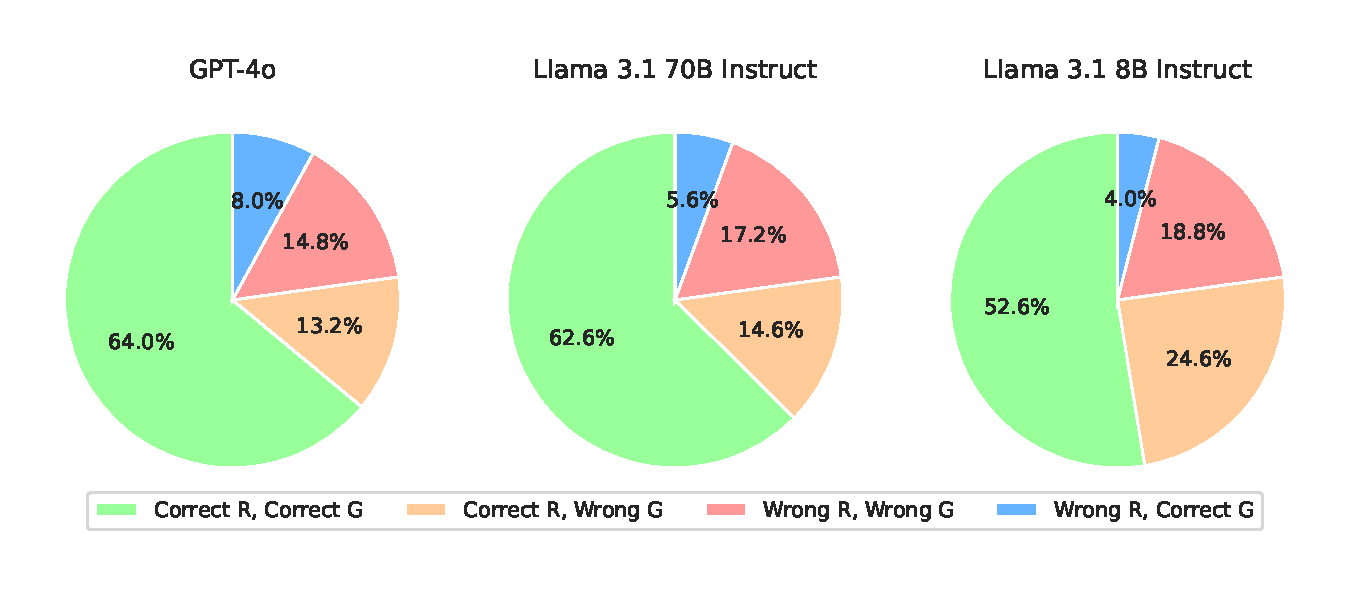
\includegraphics[width=0.9\textwidth]{figures/error_distribution.pdf} 
 \vspace{-4mm}
 \caption{An analysis of the error distribution of different reader models. We use R and G to indicate correct Recall@10 and correct answer based on the top-10 retrieved results.}
 \label{fig:error-analysis}
\end{figure}

